\documentclass[]{report}
\usepackage{amsmath, amsfonts, physics}
\usepackage{graphicx}

% Title Page
\title{MA5678 Assignment: Stage 1}
\author{David Blair}


\begin{document}
	\maketitle
	
	\section{Chosen Model}
	I have chosen to investigate the biological applications of numerical solutions to differential equations. I will be looking at the logistic equation: 
	
	\begin{align}
		\dot X(t) = rX(t)\left(1 - \frac{X(t)}{K}\right)	
		\label{eq:logistic_growth}	
	\end{align}

	Where $t \in [0, \infty)$ represents time and $X: [0, \infty) \rightarrow \mathbb{R}$. $r$ is the difference between the birth rate $b$ and the death rate $d$ where $r = b - d$. 
	$K$ represents the carrying capacity of the population. As $X(t)$ gets closer to $K$, $\dot X(t)$ decreases until it reaches 0 at $X(t) = K$.
	
	\section{Analytical Solution}
	We begin with our logistic equation, letting $X(t) = X$ and $\dot X(t) = \dot X$:
	
	\begin{align}
		\dot X = \frac{dX}{dt} = rX\left(1 - \frac{X}{K}\right)		
	\end{align}

	Firstly we separate the variables and integrate:
	
	\begin{align}
		\int\frac{1}{X\left(1 - \frac{X}{K}\right)} dX = \int r \hspace{2pt} dt
	\end{align}

	We can modify our integrand slightly:
	
	\begin{align}
		\frac{1}{X\left(1 - \frac{X}{K}\right)} = \frac{K}{X(K - X)} = \frac{1}{X} + \frac{1}{K - X}
	\end{align}

	Allowing us to determine the integral:
	
	\begin{align}
		\int\frac{1}{X\left(1 - \frac{X}{K}\right)} dX &= \int \frac{1}{X} dX + \int \frac{1}{K - X} dX \\
		&= ln|X| - ln|K - X| \\
		&= ln\left|\frac{X}{K - X}\right| = rt + C 
	\end{align}
	
	We can then rearrange the equation to get rid of the natural log:
	
	\begin{align}
		ln\left|\frac{K - X}{X}\right| &= -rt - C \\
		\frac{K - X}{X} &= e^{-rt - C} \\
		&= Ae^{-rt} \hspace{2pt} (A = \pm e^{-C})
	\end{align}
	
	If we set $t = 0$ and $X = X_0$ we can determine the value of $A$ as:
	
	\begin{align}
		A = \frac{K - X_0}{X_0}
	\end{align}

	Giving us the expression for $X(t)$:
	
	\begin{align}
		X(t) = \frac{K}{1 + Ae^{-rt}} \hspace{2pt} \text{where} \hspace{2pt} A = \frac{K - X_0}{X_0}
	\end{align}

	To plot this function, we first set $K = 100$ and $X_0 = 10$. We then take different growth rates with some being negative and some positive 
	in order to observe different behaviour:
	
	\begin{figure}[h]
		\centering
		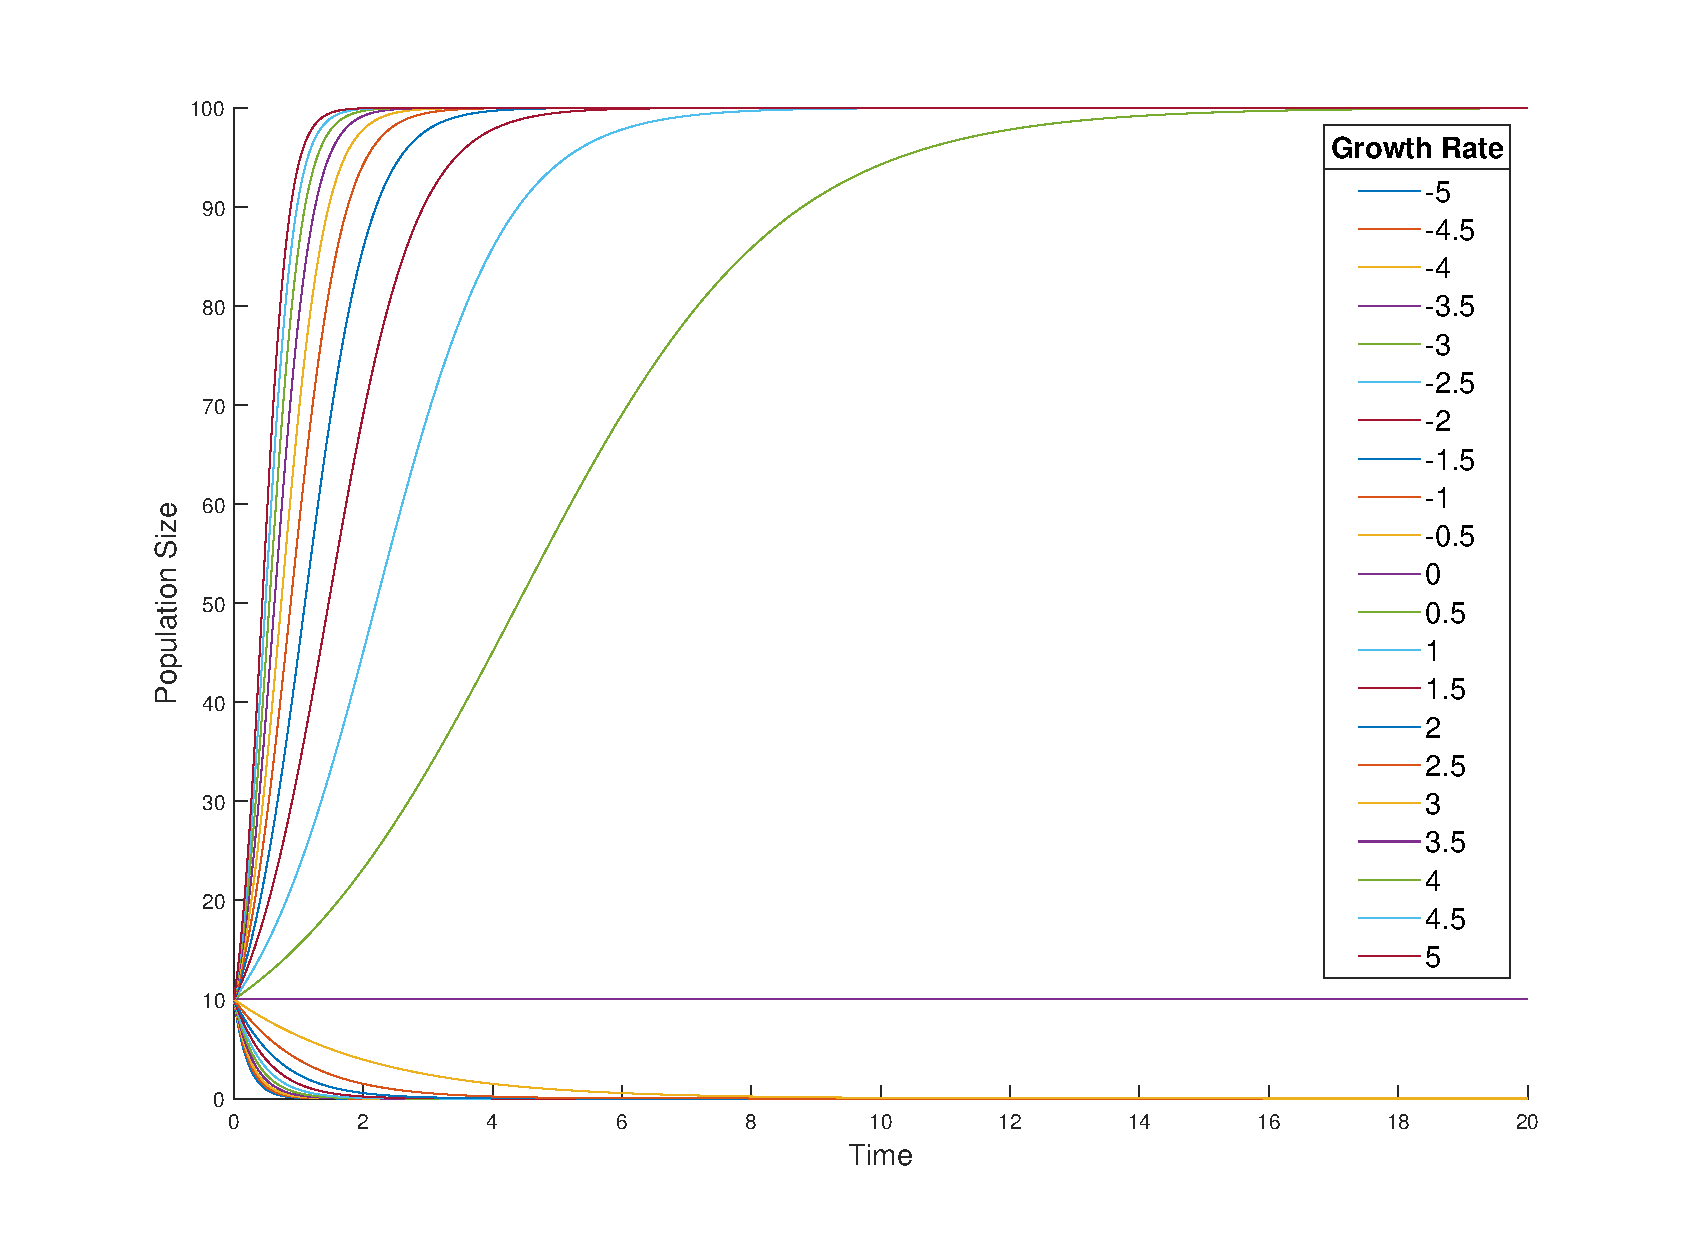
\includegraphics[scale = 0.35]{logistic_model.eps}
		\caption{Logistic Models with Varying Growth Rates}
	\end{figure}

	When the growth rate is 0, the population doesn't change. A negative growth rate will force the population to tend towards 0 and those 
	rates with a higher magnitude will reach 0 faster. Similarly, a positive growth rate will lead to an exponential growth in the population 
	before it slows down as it reaches the carrying capacity. A rate with a higher magnitude will induce a much faster exponential growth before it 
	reaches the carrying capacity.
	
	\section{Logistic Stochastic ODE}
	The logistic equation given in equation \ref{eq:logistic_growth} has an equivalent logistic stochastic ODE:
	
	\begin{align}
		dX = rX(t)\left(1 - \frac{X(t)}{K}\right)dt + \sigma X(t)dW
		\label{eq:logistic_stochastic}
	\end{align} 

	Where $X(t)$ is the population, $r$ is the intrinsic growth, $\sigma$ is the volatility and $dW$ is a Wiener process (the probabilistic element of equation \ref{eq:logistic_stochastic}). The complexity of the solution to this ODE means that we will be using a simpler approximation to run our simulations: 
	
	\begin{align}
		X_k - X_{k - 1} = rX_{k - 1}\left(1 - \frac{X_{k - 1}}{K}\right)\Delta t + \sigma X_{k - 1}\epsilon (k - 1)\sqrt{\Delta t}, \hspace{2pt} 1 \leq k \leq N
	\end{align}

	Where $\Delta t$ is the discrete time-step, $\epsilon (k - 1) \in \mathcal{N}(0, 1)$ is a random number drawn at every time step and $\sigma$ is the volatility. The initial value of the population is $S_0$. $N$ is the number of steps of the simulation. $N \Delta t = T$ where $T$ is the time horizon of the run. 
	
	To run this function, we set $N = 90$, $X_0 = 30$, $K = 20$ and $r = 0.05$. The volatility $\sigma \in \{-0.2, -0.1, 0, 0.1, 0.2\}$ and the time horizon $T \in \{80, 120\}$. Below is a plot of our stochastic model:
	
	\begin{figure}[h]
		\centering
		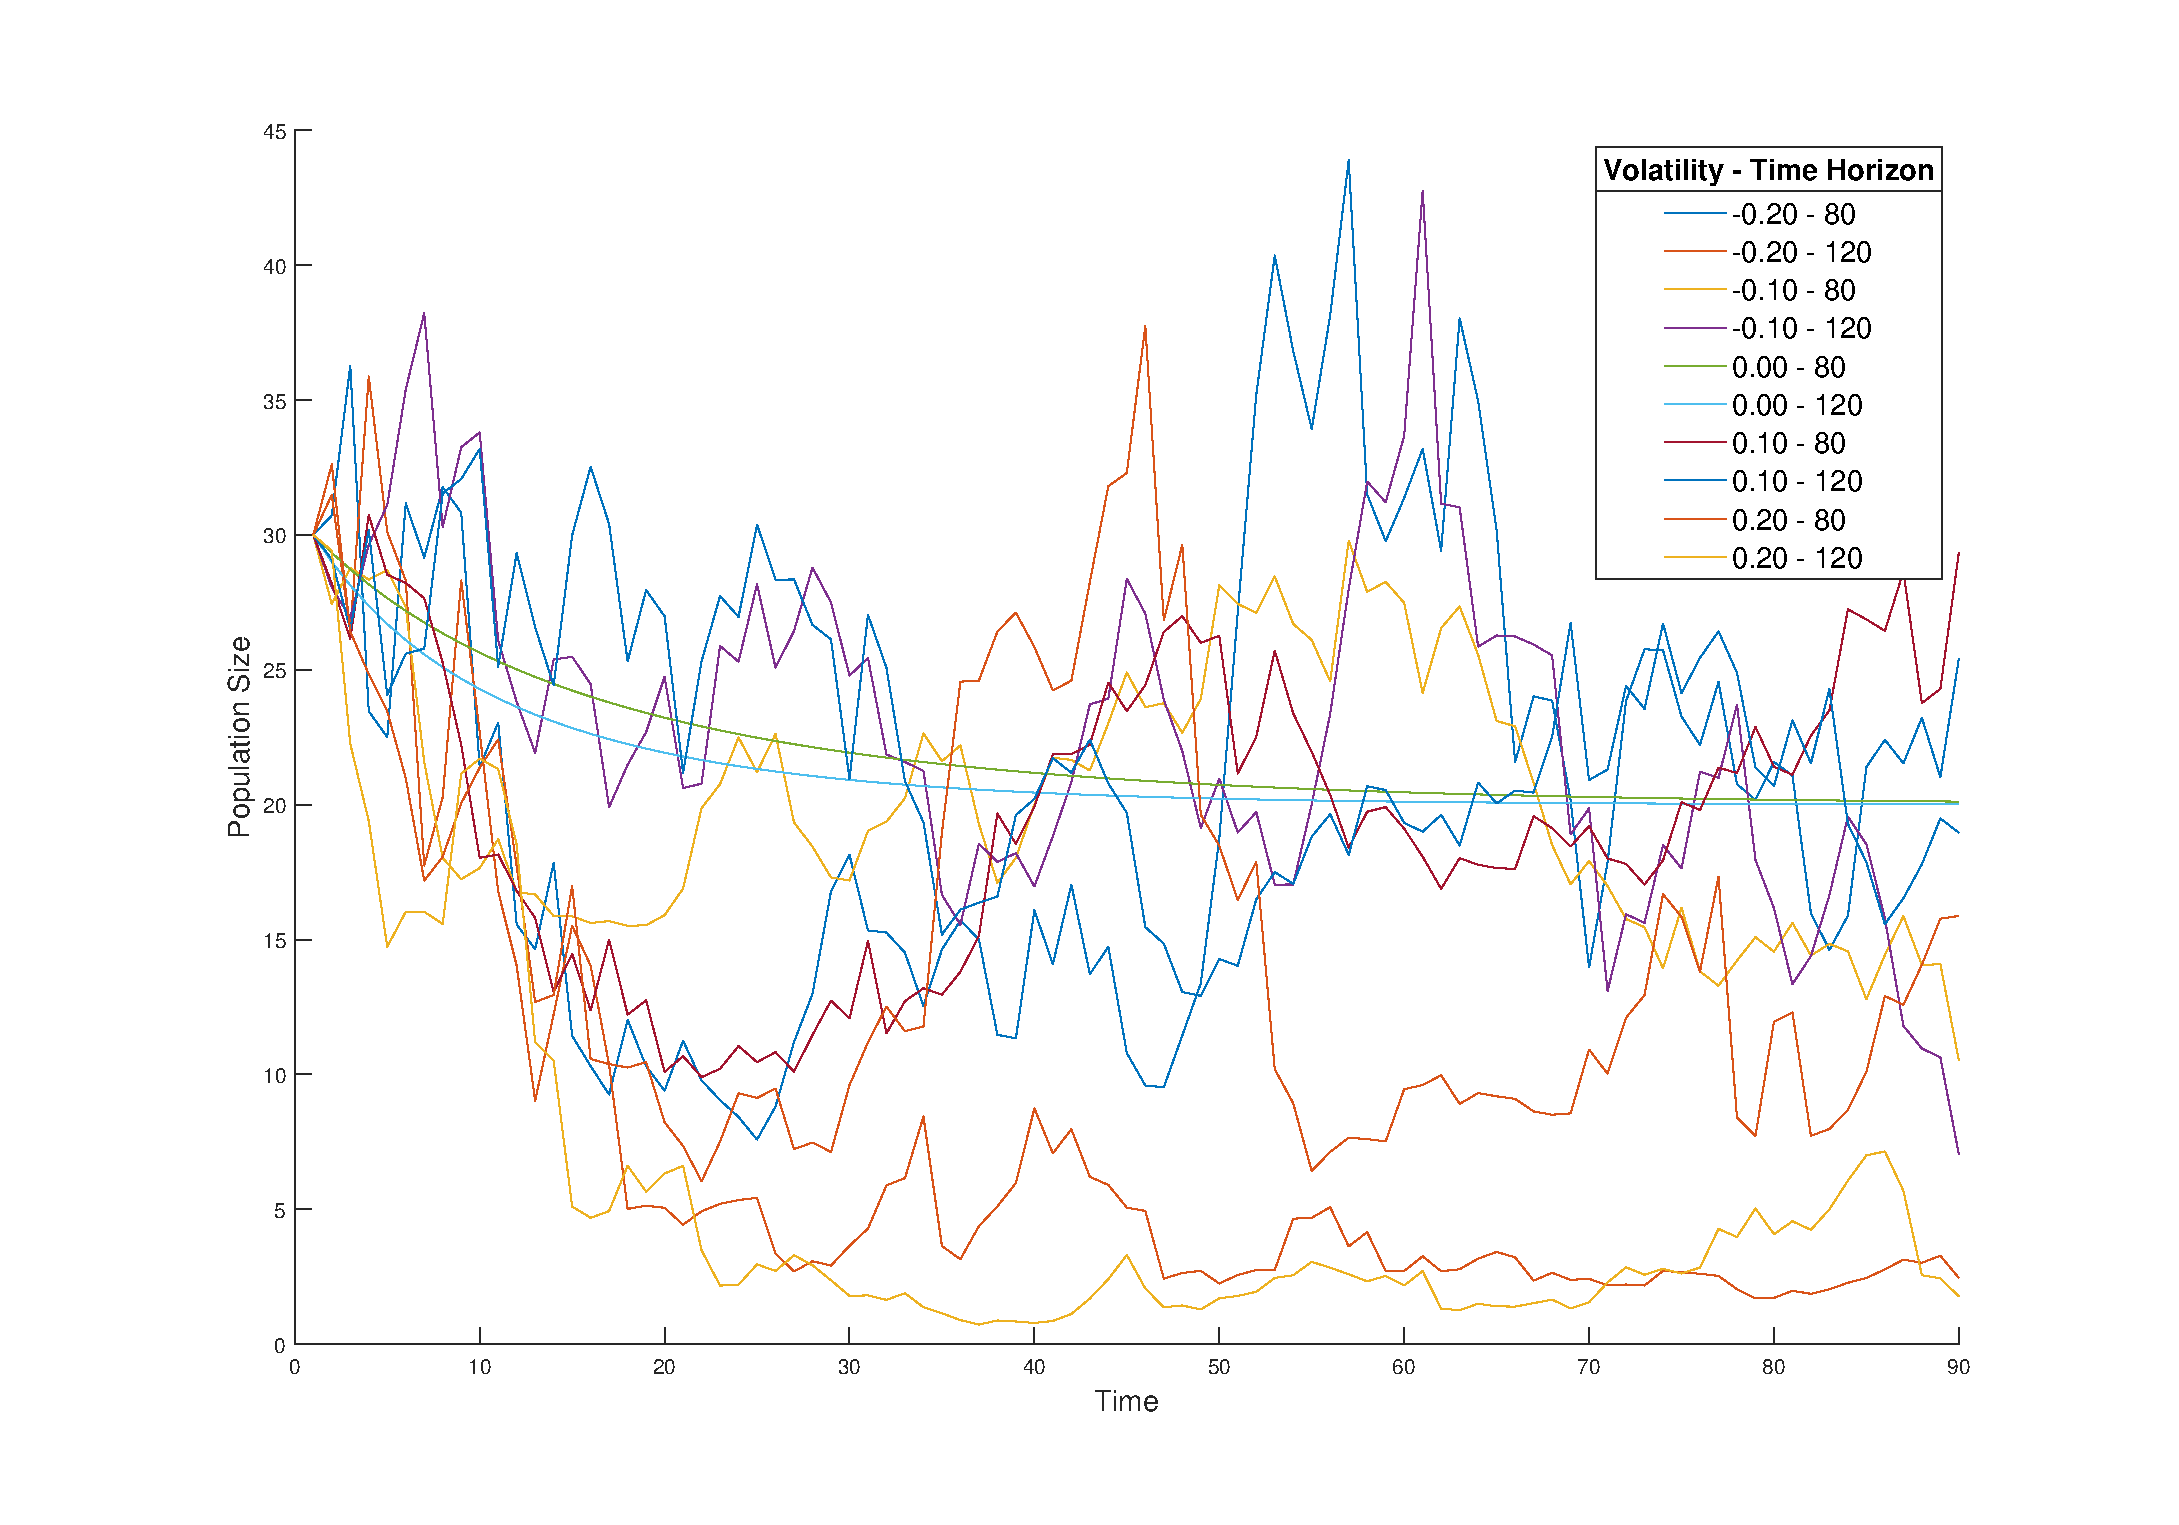
\includegraphics[scale=0.29]{stochastic_model.eps}
		\caption{Stochastic Model at Different Values of $T$ and $\sigma$}
	\end{figure}

	When we set $\sigma = 0$, it is clear that a lower time horizon results in a shallower curve which has no fluctuation. A higher magnitude in the volatility results in greater fluctuations around the initial value line.
	
	Each time we run the simulation, we are using a random number generator to sample from a normal distribution. Because of this, its slightly harder to extract meaningful information as to the effect of varying our volatility and time horizon. If we ensure that the seed we use to generate these random numbers stays the same across simulations, the random numbers selected at each step become constants and we get some interesting results:
	
	\begin{figure}[h]
		\centering
		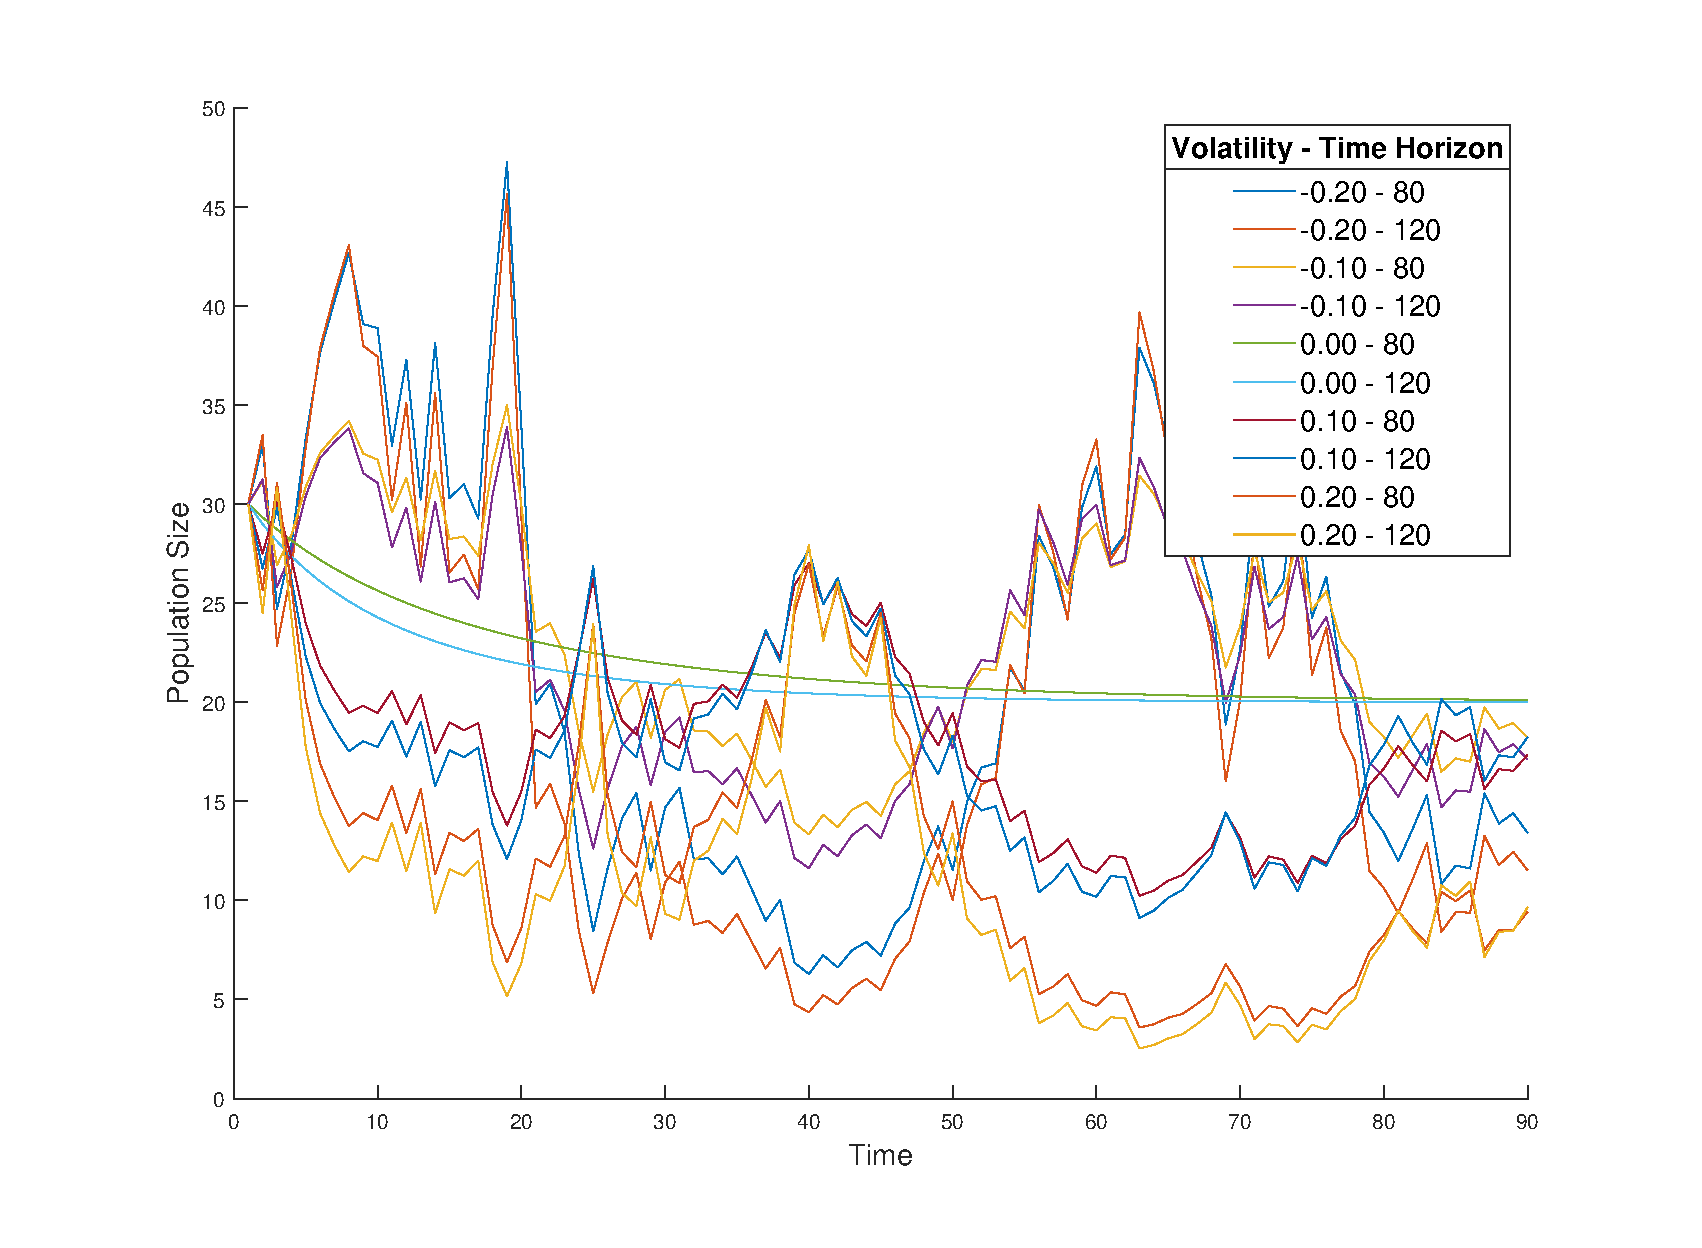
\includegraphics[scale=0.35]{stochastic_model_const.eps}
		\caption{Stochastic Model at Different Values of $T$ and $\sigma$ with Constant Seed Across Runs}
	\end{figure}
\end{document}          
